\documentclass[12pt,a4paper]{article}
\usepackage[utf8]{inputenc}
\usepackage[french]{babel}
\usepackage[T1]{fontenc}
\usepackage{mathtools}
\usepackage{amsfonts}
\usepackage{amssymb}
\usepackage[pdftex]{graphicx}
\usepackage{comment}
\usepackage{csquotes}
\usepackage{caption}
\usepackage[colorinlistoftodos,prependcaption,textsize=tiny]{todonotes}
\usepackage[left=2cm,right=2cm,top=2cm,bottom=2cm]{geometry}
\author{Angelo Ortiz}
\title{Rapport du Projet 2I013}
\graphicspath{ {../img/} }

\begin{document}
\begin{titlepage}
  \centering
  
\includegraphics[width=0.30\textwidth]{../img/logo.jpg}\par\vspace{1cm}
  {\scshape\LARGE Sorbonne Universit\'e\par}
  \vspace{1cm}
  {\scshape\Large 2I013 : Projet (application)\par}
  \vspace{1.5cm}
  {\Large \bfseries Sujet :\par}
  {\huge\bfseries IA Football\par}
  \vspace{2cm}
  {\Large\itshape Fangzhou Ye\par}
  {\Large\itshape Angelo Ortiz\par}
  \vfill
  
  % Bottom of the page
  {\large Licence d'Informatique\par}
  {\large Ann\'ee 2017/2018\par}
\end{titlepage}
 
%\newpage
\tableofcontents
\listoffigures
\newpage
  
\part*{Introduction}
\section*{Pr\'esentation}
L'unit\'e d'enseignement 2I013 consiste en un projet d'application des 
connaissances en programmation et de d\'ecouverte de nouveaux algorithmes. La 
th\'ematique du 
projet du groupe 1 a \'et\'e le football.

Le jeu comporte un terrain, deux \'equipes de joueurs et une 
balle. \'Etant donn\'e qu'une grille rectangulaire sous forme matricielle, 
c'est-\`a-dire discr\`ete, n'\'etait pas envisageable, un rep\`ere 
orthonorm\'e a \'et\'e choisi comme repr\'esentation du terrain. Pour ce faire, 
il y a deux droites en plus des axes qui d\'elimitent la surface du terrain.

\begin{figure}[!h]
  \centering
  \captionsetup{justification=centering}  
  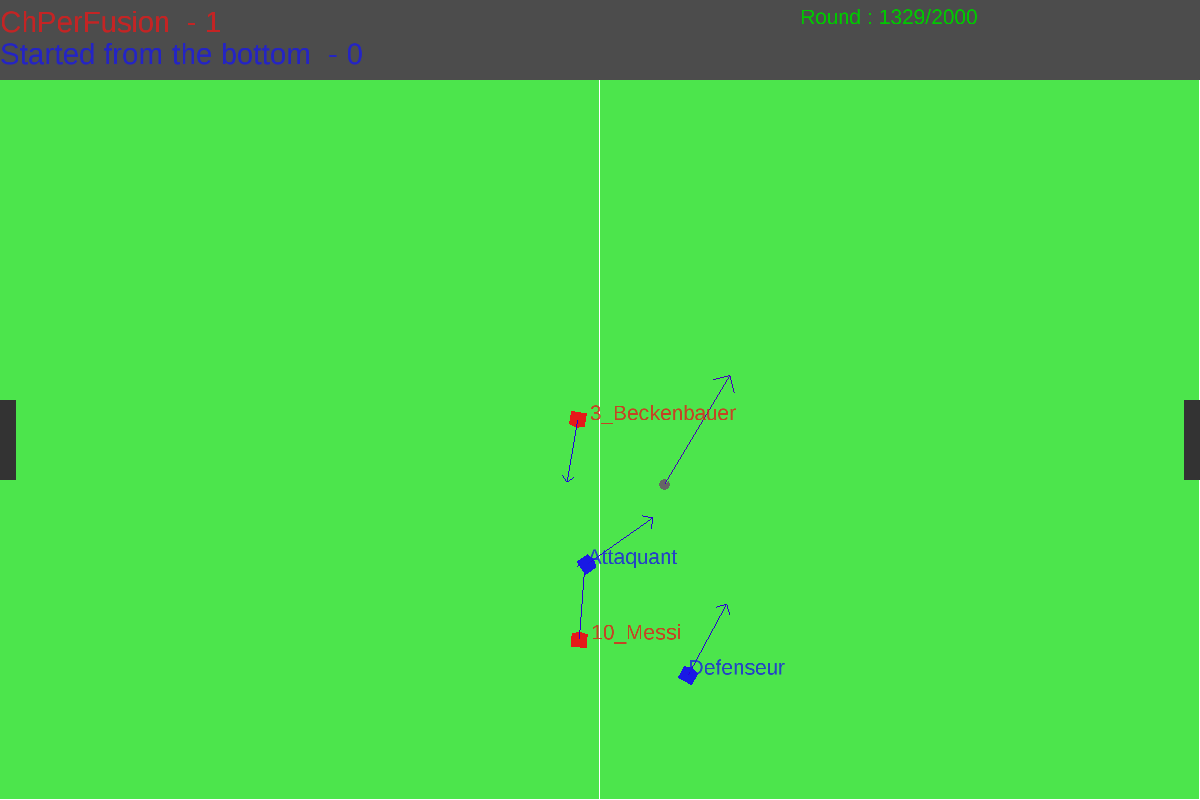
\includegraphics[width=0.7\textwidth]{apercu}
  \caption[Un aper\c{c}u du jeu]{Voici un aper\c{c}u du simulateur de football 
  lors d'une partie de notre \'equipe {\itshape ChPerFusion} en rouge face \`a 
  l'\'equipe d'un de nos camarades de classe.}
  \label{fig:apercu}
\end{figure}

Les r\`egles du football ont \'et\'e l\'eg\`erement simplifi\'ees dans le cadre 
du projet. En effet, il n'existe pas de notion de touche, mais de rebond : la 
balle ne peut pas sortir du terrain et elle choque \'elastiquement dans les 
bordures. Par ailleurs, les objets physiques du jeu, \`a savoir les joueurs et 
la balle, sont intangibles. Ceci veut dire que la balle peut passer \`a travers 
les joueurs sans modifier sa direction. C'est le cas notamment lorsque le 
joueur d\'ecide de ne pas frapper.

Pour rendre le jeu plus r\'ealiste, la notion de frottement \`a \'et\'e prise 
en compte, ce qui facilite le contr\^ole de la balle aux joueurs.
Le moteur du jeu g\'erant toutes ces r\`egles et les interactions entre les 
objets a \'et\'e fourni.

\section*{Objectifs}
L’objectif du module a \'et\'e d'apprendre \`a bien mener un projet long 
sur un nouvel environnement de d\'eveloppement, \`a savoir 
Python. 
Sachant que travail \`a \'et\'e fait en bin\^ome, on a eu besoin d'un outil 
collaboratif, en l'occurrence {\bfseries git} qui est un logiciel de gestion de 
versions d\'ecentralis\'e. 
On a ainsi appris \`a g\'erer l'avancement d'un projet \`a travers la m\'ethode 
par fonctionnalit\'es.

Le travail a consist\'e \`a d\'evelopper des intelligences artificielles 
dirigeant la prise de d\'ecisions des joueurs pour r\'eussir au mieux les 
matches dans les cat\'egories \`a un, deux et quatre joueurs.

\addcontentsline{toc}{part}{Introduction}
\newpage

\part{Architecture logicielle} %et demarche
Dans cette premi\`ere partie, on vous expliquera les choix faits 
concernant l'architecture logicielle.

Le projet a \'et\'e organis\'e en un module {\bfseries ia} 
contenant les fichiers sources de nos joueurs, un r\'epertoire regroupant les 
diff\'erentes versions des param\`etres et en divers fichiers ex\'ecutables 
permettant de lancer les algorithmes d'optimisation.

\begin{figure}[!h]
  \centering
  \captionsetup{justification=centering}
  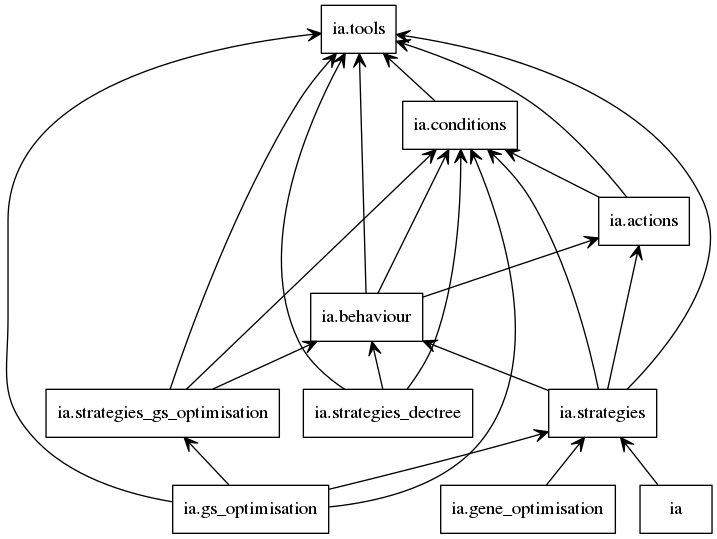
\includegraphics[width=0.8\textwidth]{packages_IA}
  \caption[La structure du module]{La structure de notre module {\bfseries ia} 
	d\'evelopp\'e tout au long du semestre}
  \label{fig:diag_classes}
\end{figure}

\section{Module de base}
Au tout d\'ebut du projet, on a r\'ealis\'e une analyse approfondie des 
fonctionnalit\'es \`a impl\'ementer et de la structure du simulateur fourni. On 
a conclu qu'il \'etait imp\'eratif de s\'eparer les fonctions et classes en 
plusieurs fichiers pour mieux les rep\'erer. On comptait ainsi de base 
quatre fichiers.

Dans le fichier {\itshape tools}, on a regroup\'e une classe enveloppe 
facilitant l'acc\`es aux informations d'un \'etat de jeu donn\'e et des 
fonctions utilitaires, par exemple, des impl\'ementations de formules 
math\'ematiques.

Puis on retrouve le fichier {\itshape conditions} qui contient toutes les 
fonctions bool\'eennes dirigeant la prise de d\'ecisions. Autrement dit, le 
comportement d'un joueur varie selon les valeurs de v\'erit\'e de ses 
conditions associ\'ees.

On passe ensuite au c\oe ur du module, \`a savoir le fichier {\itshape 
actions}. On y retrouve les actions de base qu'un joueur peut effectuer comme 
frapper, faire une passe ou revenir vers la cage.

On a vu ces fichiers grossir au fur et \`a mesure que le projet avan\c{c}ait, 
notamment {\itshape actions}. On s'est alors vu contraints 
d'ajouter un autre fichier pour am\'eliorer la structure de base. C'est ainsi 
que le fichier {\itshape behaviour} est apparu. Il contient en effet des 
super-actions, i.e.\ le comportement d'un joueur pour une phase du jeu 
donn\'ee, par exemple, la situation d'attaque avec la possession du ballon.

Par ailleurs, on communique la prise de d\'ecisions de nos joueurs au 
simulateur du jeu au moyen des classes appel\'ees strat\'egies. Celles-ci sont 
incluses dans le fichier de m\^eme nom. Ces strat\'egies correspondent alors au 
comportement d'un joueur pendant plusieurs phases du jeu, c'est-\`a-dire tout 
au long d'un match.

\begin{figure}[!h]
  \centering
  \captionsetup{justification=centering}
  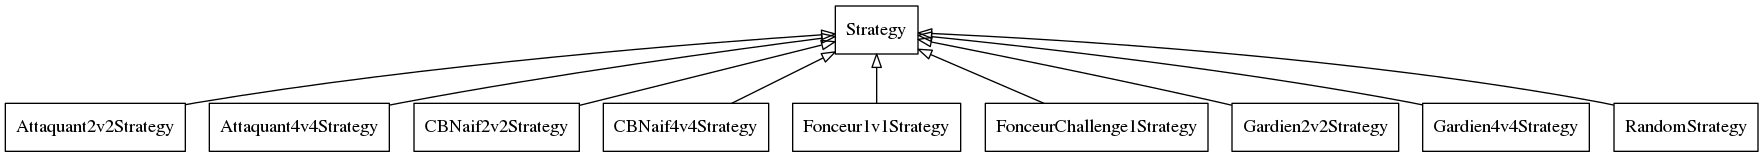
\includegraphics[width=1.\textwidth]{baseStrategies}
  \caption[Les strat\'egies de base]{Les diff\'erentes strat\'egies pour les 
\'equipes \`a un, deux ou quatre joueurs, une strat\'egie compl\`etement 
al\'eatoire et une autre pour l'unique challenge propos\'e}
  \label{fig:strats}
\end{figure}

\section{Additions chemin faisant}
Les strat\'egies con\c{c}ues ont \'evolu\'e pendant tout le semestre. On a vu 
quatre m\'ethodes d'optimisation en cours pour rendre plus intelligentes 
ces strat\'egies de base.

Pour chaque m\'ethode d'optimisation, on a eu besoin d'une classe r\'ealisant 
l'optimisation sur la base des donn\'ees recueillies soit par elle-m\^eme, soit 
par des nouvelles strat\'egies r\'eposant sur celles d\'ej\`a cod\'ees.

\begin{figure}[!h]
  \centering
  \captionsetup{justification=centering}
  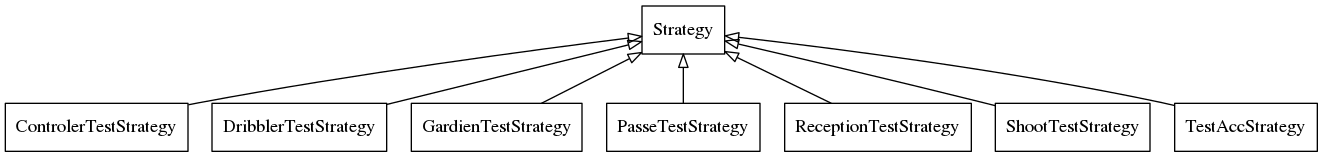
\includegraphics[width=0.9\textwidth]{gridSearch}
  \caption[Les strat\'egies pour la recherche en grille]{Les strat\'egies \`a 
am\'eliorer \`a l'aide de la recherche en grille}
  \label{fig:gs}
\end{figure}

La figure \ref{fig:gs} contient le diagramme de classes des strat\'egies 
sp\'ecialement con\c{c}ues pour la recherche en grille de param\`etres. Ces 
strat\'egies ont \'et\'e utilis\'ees par des {\itshape observateurs} des 
matches pour obtenir les valeurs optimales cherch\'ees. Les fichiers 
concern\'es par cette m\'ethode sont rep\'er\'es par le pr\'efixe 
\enquote{gs}, abr\'eg\'e du terme en anglais {\itshape grid search}.

\begin{figure}[!h]
  \centering
  \captionsetup{justification=centering}
  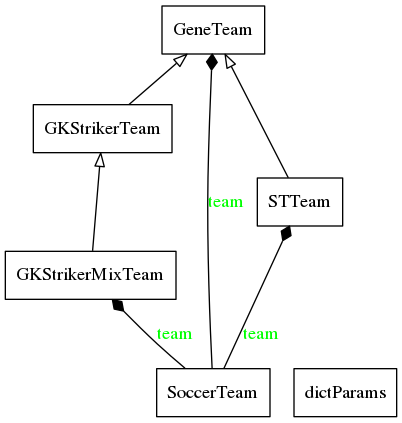
\includegraphics[width=0.6\textwidth]{genetic}
  \caption[Les classes pour l'algorithme g\'en\'etique]{Le diagramme de 
	classes pour la mise en \oe uvre d'un algorithme g\'en\'etique}
  \label{fig:gene}
\end{figure}

Pour la m\'ethode par un algorithme g\'en\'etique, on a d\'evelopp\'e deux 
classes g\'en\'eriques pour traiter le bilan des r\'esultats des strat\'egies 
de base dans plusieurs matches. On voit dans la figure \ref{fig:gene} le 
diagramme de classes r\'esultant. Le fichier cr\'ee pour cette m\'ethode 
est rep\'er\'e par le pr\'efixe \enquote{gene}.

\begin{figure}[!h]
  \centering
  \captionsetup{justification=centering}
  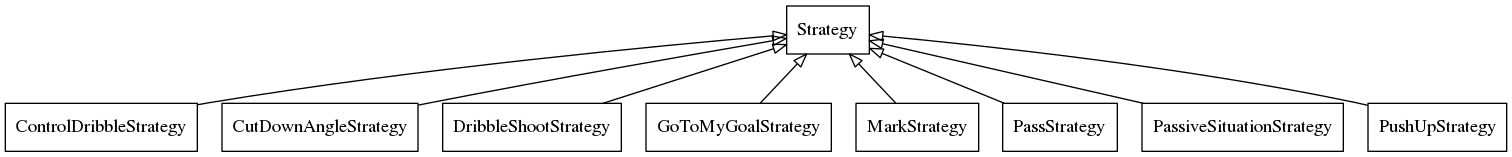
\includegraphics[width=1.\textwidth]{decisionTree}
  \caption[Les strat\'egies pour l'arbre de d\'ecision]{Les strat\'egies 
utilis\'ees pour l'application de la m\'ethode par arbres de d\'ecision}
  \label{fig:dt}
\end{figure}

La m\'ethode d'optimisation par arbres de d\'ecision est diff\'erente des 
autres en ce qui concerne la conception. En effet, la classe l'impl\'ementant 
\'etant d\'ej\`a fournie, il a suffi de d\'evelopper les strat\'egies briques 
qui allaient former une strat\'egie intelligente. Vous pouvez les apercevoir 
dans la figure \ref{fig:dt}. Le fichier contenant ces strat\'egies est 
pr\'efix\'e par \enquote{dt}, abr\'eg\'e du terme en anglais {\itshape 
decision tree}.

\begin{figure}[!h]
  \centering
  \captionsetup{justification=centering}
  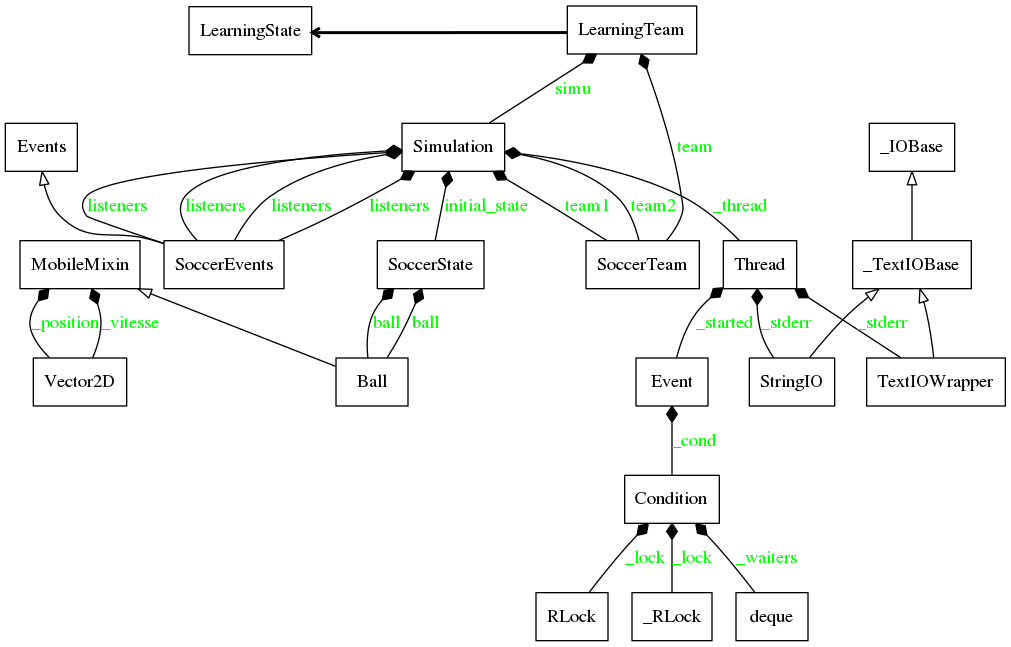
\includegraphics[width=0.8\textwidth]{machineLearning_mod}
  \caption[Les classes pour l'apprentissage automatique]{Le diagramme de 
d\'ependances des classes \texttt{LearningState} et \texttt{LearningTeam} pour 
l'impl\'ementation de l'algorithme Q-learning}
  \label{fig:ml}
\end{figure}

La derni\`ere m\'ethode d'optimisation \'etait facultative, mais on a voulu 
suivre le module jusqu'au bout. On a d\^u coder tout l'algorithme et les 
briques n\'ecessaires pour sa mise en place. Tout comme la m\'ethode 
pr\'ec\'edente, celle-ci a utilis\'e des strat\'egies briques. Par ailleurs, on 
a impl\'ement\'e l'algorithme \`a l'aide de deux classes dites 
d'{\itshape apprentissage}.
Le pr\'efixe utilis\'e pour cette m\'ethode a \'et\'e \enquote{ml}, abr\'eg\'e 
du terme en anglais {\itshape machine learning}.

\medskip
Les fichiers ex\'ecutables utilis\'es pour tester nos algorithmes 
d'optimisation se trouvent au m\^eme niveau que le module {\bfseries ia} 
pr\'efix\'es par \enquote{exe}.

\section{Librairies externes}
Il est important de rappeler que l'on compte \`a pr\'esent des nombreuses 
librairies disponibles et tr\`es souvent performantes qui ont \'et\'e le fruit 
du travail de beaucoup d'informaticiens avant nous. Ceci dit, on doit remarquer 
que l'on en a utilis\'e quelques-unes durant le d\'eveloppement du projet. On 
peut citer notamment {\itshape math}, puisque la physique du jeu comporte un 
gros composant math\'ematique ; {\itshape random}, en raison de notre 
engouement pour l'al\'eatoire ; {\itshape pickle} pour la s\'erialisation des 
donn\'ees ; {\itshape os.path} pour l'acc\`es au syst\`eme de fichiers de 
l'ordinateur ; et {\itshape numpy} pour les op\'erations simplifi\'ees sur les 
tableaux.

\newpage

\part{M\'ethodes d'optimisation}
Dans cette deuxi\`eme partie, on vous pr\'esente les diff\'erents 
algorithmes appris tout au long du semestre pour am\'eliorer 
les strat\'egies propos\'ees.

\section{Recherche en grille}
Il s'agit de la premi\`ere m\'ethode d'optimisation pre\'esent\'ee en cours. 
Elle a \'et\'e utilis\'ee pour l'optimisation d'une action.

Tout d'abord, on doit d\'efinir l'action \`a optimiser et le crit\`ere 
d'optimalit\'e, et rep\'erer les $n$ param\`etres associ\'es. Ces param\`etres 
r\'eels sont d\'enot\'es $x_i$, avec $i=1,\dotsc,n$. Le crit\`ere 
d'optimalit\'e correspond alors \`a la fonction $f: \mathbb{R}^n \to \{0,1\}$.

Puis on obtient l'ensemble $\mathbb{E}_i$ de valeurs possibles pour chaque 
param\`etre. 
Pour les param\`etres discrets, il suffit d'utiliser l'ensemble fini des valeurs 
qu'il peut prendre. 
Quant aux param\`etres continus, on compte un intervalle ferm\'e $I_i$ de 
valeurs possibles pour chaque $x_i$. Il est alors n\'ecessaire de faire en 
amont une discr\'etisation, i.e.\ on divise l'intervalle selon un pas de 
pr\'ecision. La fonction se transforme alors en $f: \mathbb{E} \to \{0,1\}$, 
o\`u $\mathbb{E} =  \mathbb{E}_1 \times \cdots \times \mathbb{E}_n$.

On fait ensuite une recherche exhaustive sur tout l'espace de 
points $\mathbb{E}$ : on teste chaque vecteur $x \in \mathbb{E}$ sous 
diff\'erents conditions environnementales et on moyenne les \'evaluations par 
$f(x)$ dans lesdites conditions. Finalement, on prend la valeur optimale et son 
vecteur $x$ associ\'e.

Il est important de remarquer que la plupart de nos param\`etres sont continus. 
Pour obtenir des valeurs plus pr\'ecises et un meilleur comportement, on a 
besoin d'un pas de discr\'etisation tr\`es petit. De ce fait, 
$|\mathbb{E}| \gg 1$. \`A cause des longs temps d'ex\'ecution, on a 
d\'ecid\'e que l'algorithme mis en place ne convenait pas \`a moyen terme.

\section{Algorithmes g\'en\'etiques}
Dans un deuxi\`eme temps, on est pass\'es \`a une m\'ethode heuristique au 
lieu d'une recherche exhaustive de l'espace de repr\'esentation. En effet, 
une solution approch\'ee est suffisante dans un certain intervalle de 
confiance. Ceci a donn\'e lieu \`a la mise en place d'une impl\'ementation 
d'algorithme g\'en\'etique pour optimiser toutes nos \'equipes.

Cette classe d'algorithmes se base sur la th\'eorie de l'\'evolution. En effet, 
la notion de s\'election naturelle est le m\'ecanisme permettant de choisir des 
solutions potentielles de plus en plus meilleures.

La toute premi\`ere chose \`a faire est la d\'efinition de la fonction 
$f: \mathbb{R}^n \to \mathbb{E}$ \`a optimiser, o\`u $n$ est le nombre de 
param\`etres concern\'es. Un \'el\'ement $x=(x_1,\dotsc,x_n) \in \mathbb{R}^n$ 
est appel\'e {\itshape candidat} ou {\itshape chromosome}, et chacune de ses 
coordonn\'ees $x_i$ avec $i=1,\dotsc,n$, appel\'ee {\itshape propri\'et\'e} 
ou encore {\itshape g\`ene}, correspond \`a un param\`etre \`a optimiser. Elles 
forment le {\itshape g\'enotype}.
Autrement dit, un candidat correspond \`a une \'equipe d\'efinie par les valeurs
de ses propri\'et\'es.

Dans le cadre du projet, on a d\'efini $f(x)=(V,N,D,P,C)$ comme le 
bilan apr\`es avoir disput\'e plusieurs matches avec les m\^emes valeurs des 
param\`etres donn\'ees par $x$, i.e.\ le tuple compos\'e du nombre de 
victoires, matches nuls, d\'efaites, buts marqu\'es et buts encaiss\'es. La 
relation d'ordre suit les r\`egles du classement d'un tournoi de football.
De plus, l'ensemble $\mathbb{R}^n$ a \'et\'e r\'eduit \`a $I_1 \times 
\dotsm \times I_n$, avec $I_i$ l'intervalle de valeurs optimales pour le 
param\`etre $x_i$ pour chaque $i = 1,\dotsc, n$.

Cette classe d'algorithmes comportent quatre \'etapes.

\begin{enumerate}
  \item \underline{Initialisation :} Tout d'abord, il faut g\'en\'erer un 
  ensemble de candidats $\{x_1,\dotsc,x_m\}$. Le but est d'obtenir une 
  population initiale la plus diverse possible de sorte \`a pouvoir atteindre 
le plus de maxima relatifs. C'est pourquoi cette premi\`ere g\'en\'eration est 
obtenue de mani\`ere al\'eatoire.
  \item \underline{\'Evaluation :} Ensuite, on \'evalue la fonction en 
  chacun des candidats, i.e.\ on calcule $\{f(x_1),\dotsc,f(x_m)\}$.
  \item \underline{S\'election :} Suivant la notion de s\'election 
  naturelle, on ne conserve que les candidats avec les meilleurs r\'esultats. 
  Autrement dit, on dresse un classement des \'equipes associ\'ees aux 
  candidats et n'en garde qu'une partie.
  \item \underline{Reproduction :} Finalement, on attribue les places 
  libres aux candidats n\'es du brassage g\'en\'etique des candidats les 
  plus performants. Pour ce faire, on compte sur deux m\'ethodes, \`a savoir le 
  croisement et la mutation. \'Etant donn\'e deux parents, on commence par les 
  cloner en deux enfants. Puis on choisit une ligne de coupe divisant le 
  g\'enotype en deux parties. Ensuite, les enfants s'\'echangent une partie de 
  leur g\'enotype. Le croisement s'arr\^ete \`a ce stade-l\`a, tandis que la 
  mutation ajoute du bruit al\'eatoirement dans un g\`ene pour chacun 
  des nouveaux chromosomes. On a d\'ecid\'e de faire une petite modification 
  \`a cette \'etape-l\`a lors de l'impl\'ementation pour avoir encore plus de 
  diversification : une minorit\'e des places libres est attribu\'ee \`a des 
  candidats g\'en\'er\'es al\'eatoirement.
\end{enumerate}

Cet algorithme \'etant it\'eratif, on recommence \`a la deuxi\`eme phase avec 
la nouvelle g\'en\'eration. Au bout d'un nombre raisonnable d'it\'erations, on 
se retrouve avec une g\'en\'eration compos\'ee de chromosomes tr\`es proches 
des maxima relatifs. On finit donc l'algorithme par prendre le candidat optimal 
de la derni\`ere population.

Cette m\'ethode a permis d'am\'eliorer nos \'equipes progressivement et les 
valeurs de tous les param\`etres mis en place ont \'et\'e d\'efinies au moyen 
de nombreuses ex\'ecutions de cette m\'ethode.

\section{Apprentissage automatique}
Dans la derni\`ere partie du semestre, on s'est concentr\'es sur 
l'apprentissage automatique. Les enseignants ont pr\'esent\'e les deux grandes 
familles d'algorithmes d'apprentissage : supervis\'es et non supervis\'es, ainsi 
que l'apprentissage par renforcement. Deux m\'ethodes ont \'et\'e 
impl\'ement\'ees lors du projet.

\subsection*{Arbres de d\'ecision (de classification)}
Il s'agit d'une technique d'apprentissage supervis\'e. Pour l'appliquer, on 
a besoin d'un {\itshape espace de repr\'esentation} $\mathcal{X}$, d'un 
ensemble d'{\itshape \'etiquettes} ou {\itshape classes} $Y$ et d'une liste de 
$m$ exemples d'apprentissage $(x^i,y^i)$, o\`u $x^i \in \mathcal{X}$, $y^i \in 
Y, i = 1,\dotsc,m$, appel\'ee {\itshape ensemble d'apprentissage}.
Le but de cette technique est de trouver une fonction $f: \mathcal{X} \to 
Y$ telle que l'on puisse pr\'edire \`a quelle classe appartient une 
future variable $x \in \mathcal{X}$.

Concr\`etement, on veut associer une certaine action \`a chaque \'etat du jeu. 
Comme les informations contenues dans les \'etats du jeu ne sont pas 
g\'en\'eralisables dans l'\'etat, on utilisera une repr\'esentation par $n$ 
caract\'eristiques g\'en\'eralis\'ees qui pr\'ecisent la configuration du 
terrain. On a ainsi que $\mathcal{X} = \mathbb{R}^n$, avec $n$ la dimension de 
l'espace de repr\'esentation. De plus, l'ensemble d'\'etiquettes devient 
l'ensemble d'actions possibles $A$. On veut donc trouver une fonction $f: 
\mathbb{R}^n \to A$ qui fournit la meilleure action possible pour tout \'etat du 
jeu.

Le probl\`eme auquel on est confront\'es se r\'eduit alors \`a 
partitionner l'espace de repr\'esentation en $p=|A|$ parties 
$\mathcal{X}_1,\mathcal{X}_2,\dotsc,\mathcal{X}_p$ de sorte que 
$f([\mathcal{X}_i]) = \{ a_i \} \subset A$, $i = 1,\dotsc,p$. On utilise les 
arbres de d\'ecisions pour repr\'esenter ce partionnement. Ceci 
implique que chaque n\oe ud interne correspond \`a un test sur une des $n$ 
dimensions de $\mathcal{X}$ et que chaque feuille correspond \`a l'action \`a 
entreprendre pour l'\'etat donn\'e par le chemin suivi depuis la racine.

\begin{figure}[!h]
  \centering
  \captionsetup{justification=centering}
  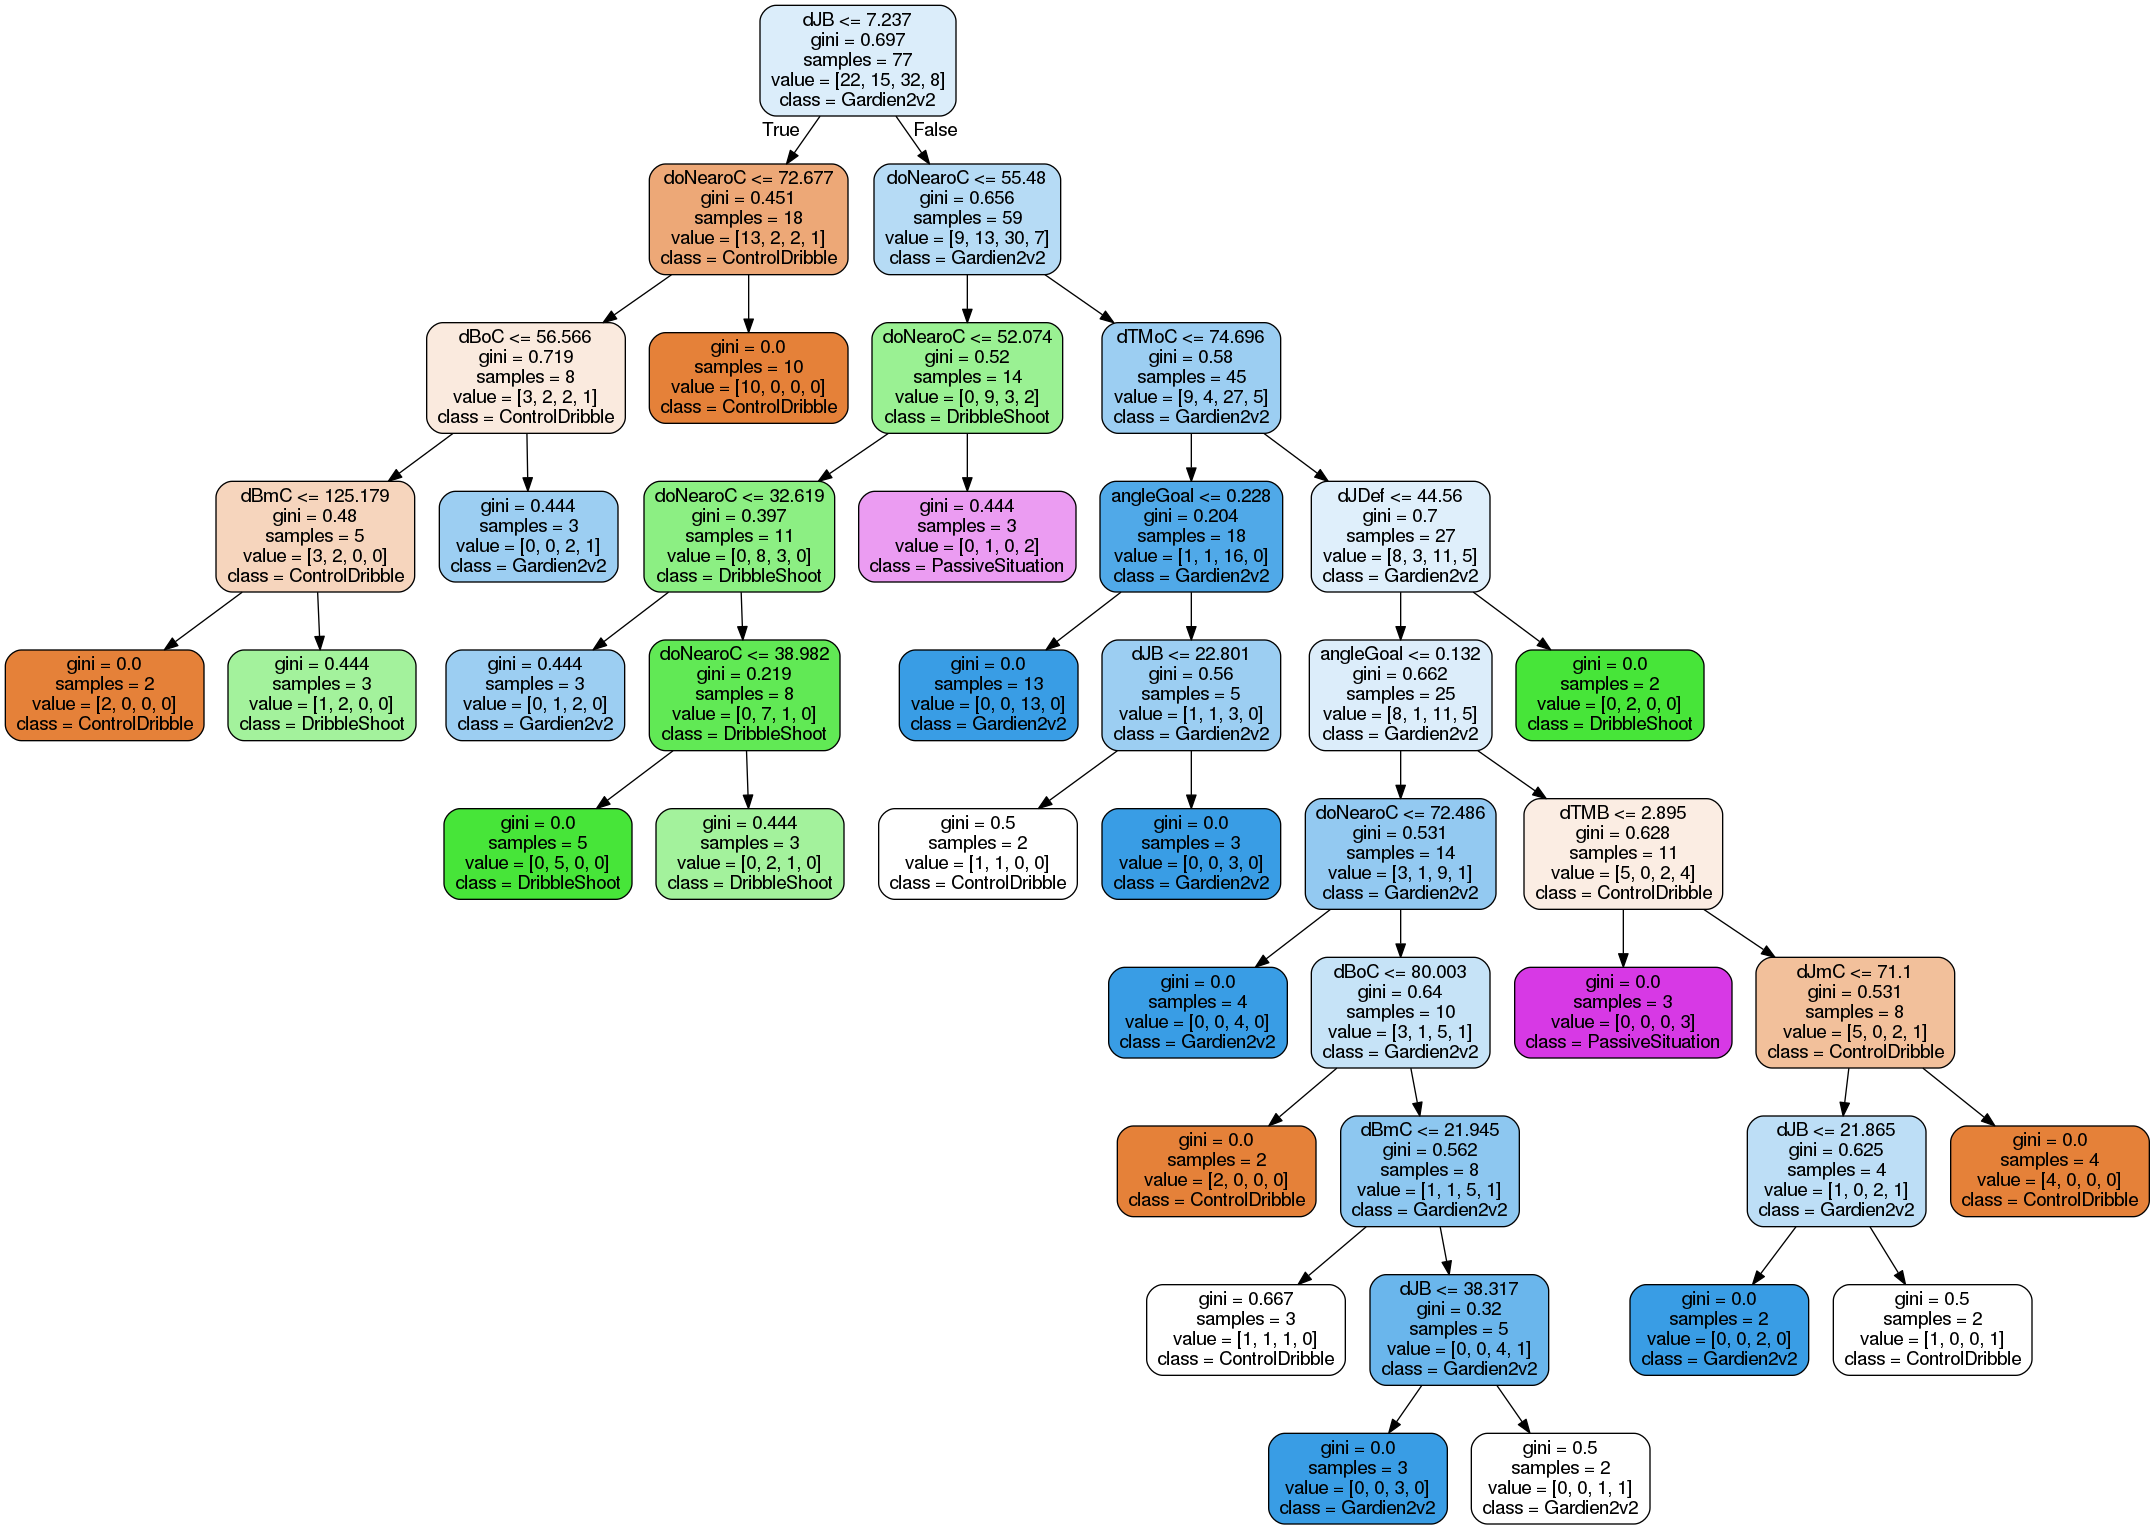
\includegraphics[width=0.8\textwidth]{dt_example}
  \caption[Un exemple d'arbre de d\'ecision]{Voici un exemple d'arbre de 
d\'ecision obtenu \`a l'issue de l'ex\'ecution de l'algorithme propos\'e}
  \label{fig:dt_ex}
\end{figure}

On nous a fourni une strat\'egie sp\'eciale \texttt{KeyboardStrategy} 
comportant les outils de base n\'ecessaires \`a la mise en place de cette 
m\'ethode, allant de la g\'en\'eration de l'ensemble d'apprentissage au 
partionnement de l'espace de repr\'esentation, en passant par l'application de 
la fonction lors des matches. 
Elle permet d'associer des touches clavier aux diff\'erentes strat\'egies de 
sorte que l'on puisse pr\'eciser la strat\'egie pr\'econis\'ee pour les 
diff\'erentes phases du jeu. Ceci conforme ce que l'on appelle l'ensemble 
d'apprentissage. Cet ensemble est trait\'e \`a l'aide des $n$ carat\'eristiques 
g\'en\'eralis\'ees d\'efinies auparavant et, \`a l'issue de ceci, on compte 
un partionnement de $\mathbb{R}^n$. Cette strat\'egie utilise alors la fonction 
$f$ lors des matches suivants, ce qui donne un comportement plus intelligent 
\`a nos joueurs.

Cette m\'ethode n'a pas \'et\'e utilis\'ee pour am\'eliorer la 
prise de d\'ecisions sur les actions parce que l'on a trouv\'e difficile 
l'interaction \`a travers le clavier pour plus de quatre actions.

\subsection*{Q-learning}
Cet algorithme d'apprentissage par renforcement r\'epose sur un ensemble 
d'\'etats $S$, un ensemble d'actions $A$, et une fonction $Q: S \times A \to 
\mathbb{R}$, appel\'ee {\itshape politique}, pond\'erant une paire form\'ee 
par un {\itshape \'etat} donn\'e et une {\itshape action} \`a entreprendre pour 
cet \'etat-ci. Cette pond\'eration est nomm\'ee {\itshape r\'ecompense}. La 
notion d'\'etat correspond \`a celle donn\'ee dans la section des arbres 
binaires de d\'ecision. Il utilise aussi la notion d'{\itshape \'episode} que 
l'on associe \`a un match dans le cadre du projet. Son principe est le suivant : 
on apprend une politique comportementale qui optimise l'esp\'erance des 
r\'ecompenses.

La phase d'initialisation consiste \`a attribuer \`a $Q$ une valeur fixe 
arbitraire, ici 0. La phase it\'erative concerne un \'episode, ou encore un 
match, et est r\'ep\'et\'ee pour les $k$ \'episodes. 
Pour un \'etat $s_t$ donn\'e, on choisit une action $a_t$ selon la politique $Q$ 
et observe la r\'ecompense $r_t$ associ\'ee \`a cette paire. Cette action 
g\'en\`ere un nouvel \'etat $s_{t+1}$. Il est \`a noter qu'il n'y a pas de 
choix concernant l'\'etat initial $s_0$, puisqu'il est toujours le m\^eme pour 
un match de football : ceci correspond au coup d'envoi. Ensuite, on met \`a 
jour la politique selon la formule ci-dessous.

\begin{equation*}
  Q(s_t,a_t) \gets (1-\alpha) \cdot 
  \underbrace{Q(s_t,a_t)}_{\mathclap{\text{valeur actuelle}}} + \ \alpha(k) 
\cdot \underbrace{\Big(r_t + \gamma \cdot \max_a(Q_{t+1},a) 
	\Big)}_{\mathclap{\text{valeur   apprise}}}
\end{equation*}

Ici, $\alpha$ repr\'esente la vitesse d'apprentissage et $\gamma$ le facteur 
d'actualisation. D'un c\^ot\'e, la vitesse d'apprentissage d\'etermine 
l'\'equilibre entre exploration et exploitation. En effet, une valeur de 
0 implique l'utilisation exclusive des choix actuels, alors qu'une 
valeur 1 ne ferait que consid\'erer le dernier r\'esultat.
Comme notre agent est cens\'e \^etre plus intelligent au fur et \`a mesure des 
\'episodes, il doit apprendre de moins en moins des it\'erations restantes. 
C'est pourquoi on a choisi une vitesse d'apprentissage polyn\^omiale, i.e.\ 
$\alpha(k)=\dfrac{1}{k^\omega}$, avec $\omega \in \left] 0,5;1 \right[$ fix\'e.

D'un autre c\^ot\'e, le facteur d'actualisation d\'etermine l'importance des 
r\'ecompenses futures. Une valeur de 0 ne prend en consid\'eration que les 
r\'ecompenses courantes, tandis qu'une valeur de 1 met en valeur les 
r\'ecompenses plus lointaines. On avait pr\'ecis\'e qu'un \'episode 
correspondait \`a un match ; par cons\'equent, la r\'eussite d'une succession 
d'actions d\'epend du r\'esultat final du match. De ce fait, on a int\'er\^et 
\`a retarder au maximum les r\'ecompenses. Ceci se traduit par le choix d'un 
facteur $\gamma$ proche de 1.

Si le nouvel \'etat $s_{t+1}$ est terminal, on passe \`a l'\'episode 
suivant. Sinon on choisit une action pour cet \'etat et refait la mise \`a jour 
de la politique.

\`A la fin de l'algorithme, on se retrouve avec une politique qui nous rend 
l'action la plus ad\'equate pour tout \'etat du jeu. \'Etant donn\'e que les 
carat\'eristiques utilis\'ees pour d\'efinir un \'etat sont continues, 
on a d\'efini des intervalles d'\'equivalence. Cela n'emp\^eche que le nombre 
total d'\'etats est \'enorme et fait donc exploser la m\'emoire. Bien 
qu'impl\'ement\'e, on ne s'est pas servi de cet algorithme pour les 
versions compl\`etement fonctionnelles de nos \'equipes de football. 

\newpage

\part{Strat\'egies}
Dans cette derni\`ere partie, on vous d\'etaille le comportement de nos 
diff\'erents joueurs.
Compte tenu de la taille du terrain de jeu, le nombre maximum de joueurs par 
\'equipe est limit\'e \`a quatre. 
Ainsi, il y a trois cat\'egories de matches 
selon le nombre de joueurs par \'equipe : un, deux ou quatre.

\section{Un joueur}
Pour l'\'equipe compos\'ee uniquement d'un joueur, on a d\'evelopp\'e un seul 
joueur que l'on appelle {\itshape Fonceur}. 

\subsection*{Fonceur}
Il s'agit du point de d\'epart du projet. Le but des premi\`eres semaines 
\'etant de se familiariser avec le code source fourni, on a cr\'e\'e une 
strat\'egie tr\`es simple et na\"ive. 
Ainsi, il faisait tout au maximum : il devait se rapprocher de la balle \`a 
toute vitesse lorsqu'il n'en avait pas la possession et il 
frappait avec toute sa puissance dans le cas contraire.
Compte tenu que ce comportement ressemblait beaucoup aux autres fonceurs de la 
classe \`a une param\'etrisation pr\`es et que les matches finissaient en nul, 
on 
a ajout\'e les fonctionnalit\'es suivantes : l'avanc\'ee balle au pied et le 
dribble.
Pour ce faire, on a utilis\'e la recherche en grille des param\`etres. En 
effet, les valeurs optimales pour la puissance du contr\^ole de la balle et 
le dribble \'etaient inconnues.
Comme on ne connaissait m\^eme pas quel \'etait le bon sous-intervalle des 
valeurs, on a commenc\'e par discr\'etiser tout l'intervalle 
de valeurs possibles $\left[0;6\right]$ avec un pas de 0,5. Puis on a 
r\'ep\'et\'e le m\^eme proc\'ed\'e pour le sous-intervalle avec les m\'eilleurs 
r\'esultats avec des pas de discr\'etisation de plus en plus petits.

Par ailleurs, on savait que la frappe \'etait plus r\'ealiste avec une 
variation sur la pr\'ecision selon les vitesses du joueur et de la balle, 
l'angle entre ces deux vecteurs et la puissance de la frappe, en plus d'un 
param\`etre al\'eatoire. C'est pourquoi on ne pouvait plus maintenir 
une puissance de frappe constante. On a donc d\'ecid\'e de la faire varier 
seulement dans le cas d'une frappe vers le but adverse. En effet, on a pris en 
consid\'eration la distance du joueur \`a la cage adverse et l'angle du vecteur 
allant de la position du joueur vers le centre de la cage adverse 
par rapport \`a l'horizontale. Ceci a donn\'e lieu \`a deux param\`etres 
optimis\'es aussi gr\^ace \`a la recherche en grille. On a utilis\'e d'ailleurs 
le m\^eme proc\'ed\'e que pour les param\`etres pr\'ec\'edents.

Cela a rapport\'e de bons r\'esultats contre les \'equipes restant 
na\"ives, mais n'a pas suffi pour battre les \'equipes plus d\'evelopp\'ees. 
En effet, il est tr\`es difficile de devancer un adversaire qui fait une 
pression de pr\`es sur le ballon de sorte que les tentatives de 
dribbles du fonceur \'echouent.
De plus, ses essais de dribble dans sa propre surface de r\'eparation 
\'etaient souvent trop faibles pour \'echapper au danger que signifie 
l'adversaire venant le presser. Il d\'egage \`a pres\'ent la balle le plus loin 
possible pour pallier cette difficult\'e.

On a ensuite trouv\'e les valeurs optimales pour tous les param\`etres en 
m\^eme temps gr\^ace \`a notre algorithme g\'en\'etique, plus pr\'ecis\'ement 
au travers de la classe \texttt{STTeam}.
Il n'emp\^eche que cette strat\'egie est rest\'ee assez basique \`a l'\'egard 
de celles de nos camarades de classe vu les r\'esultats des tournois 
hebdomadaires. 
Autrement dit, le dribble est tr\`es peu r\'eussi et les contre-attaques 
arrivent lorsque le joueur est dans sa course vers l'avant, ce qui le surprend 
et fait que l'adversaire se trouve facilement seul face \`a notre cage.

Finalement, on a voulu tester la performance de notre algorithme 
d'apprentissage par renforcement. Pour ce faire, on a d\'evelopp\'e plusieurs 
strat\'egies simples sur la base du comportement pr\'esent \`a ce moment-l\`a.
On l'a d\'eroul\'e pour le cas particulier de l'\'equipe \`a un seul joueur. On 
a bien v\'erifi\'e que l'algorithme n\'ecessite de beaucoup d'espace m\'emoire 
pour offrir des bons r\'esultats. En effet, on compte un fichier d'un peu plus 
de 400MB qui montre des indices d'un comportement plus intelligent. Cette 
optimisation n'ainsi pas \'et\'e prise en compte pour la version fonctionnelle 
de l'\'equipe \`a un joueur.

\subsection*{Cas particulier : challenge}
Au d\'ebut du semestre, les enseignants nous ont pr\'esent\'e un challenge, \`a 
savoir marquer le plus de buts en 2000 pas de temps. On a r\'eutilis\'e notre 
fonceur pour ce cas particulier. \`A ce moment-l\`a, le fonceur ne comptait que 
la frappe na\"ive. 

Puisqu'il est tr\`es peu probable que la balle rentre dans 
la cage adverse d'un seul coup, le fonceur fait son travail en deux phases. 
Tout d'abord, il frappe doucement la balle de sorte qu'elle reste dans une 
position axiale. Puis il fait une frappe plus forte pour mettre la balle au 
fond. On a aussi utilis\'e la recherche en grille pour optimiser cette 
strat\'egie. 

\section{Deux joueurs}
Cette cat\'egorie a \'et\'e celle sur laquelle on a consacr\'e la plupart du 
projet. On compte trois joueurs fonctionnels que l'on appelle 
{\itshape Attaquant}, {\itshape Gardien} et {\itshape D\'efenseur}. 

\subsection*{Attaquant}
Il a une vocation plut\^ot offensive. Son comportement initial \'etait celui 
d'un attaquant classique. Effectivement, il l'a h\'erit\'e du fonceur, \'etant 
jusqu'\`a alors optimis\'e seulement par la recherche en grille.

Sa conduite sans la balle d\'ependait de la zone dans laquelle se trouvait le 
porteur de la balle : il le pressait si l'adversaire \'etait \'eloign\'e de sa 
surface et se d\'ecalait vers les c\^ot\'es pour faciliter les contre-attaques 
dans le cas contraire. 
Quant \`a son style de jeu avec la balle au pied, il avan\c{c}ait de petites 
distances sur le terrain et frappait la balle lorsqu'il se trouvait dans la 
surface de r\'eparation adverse. Tout comme pour le fonceur, il perdait la balle 
trop facilement. 
C'est pourquoi on a ajout\'e le dribble al\'eatoire, ce qui l'a rendu 
impr\'evisible face aux tentatives adverses de lui arracher le ballon. C'est 
avec cette modification que l'on a utilis\'e pour la toute premi\`ere fois 
notre impl\'ementation d'algorithme g\'en\'etique pour optimiser la strat\'egie 
au complet. On a donc d\'evelopp\'e les classes \texttt{dictParams}, 
correspondant au dictionnaire des param\`etres, et \texttt{GeneTeam}, une 
classe g\'en\'erique permettant de lancer l'algorithme. 
Ce dictionnaire g\'erait aussi bien les valeurs des param\`etres que 
leurs intervalles optimaux. Pour les param\`etres d\'ej\`a optimis\'es par la 
recherche en grille, on a juste repris leurs intervalles optimaux. Quant aux 
autres, on a d'abord encadr\'e les valeurs de mani\`ere analytique et 
coh\'erente avec le rendu attendu. Puis on a utilis\'e de nouveau la m\'ethode 
essai et erreur pour trouver des intervalles plus petits et appropri\'es.
Pour le cas particulier de l'\'equipe \`a deux joueurs dont l'attaquant fait 
partie, on a d\'evelopp\'e la classe \texttt{GKStrikerTeam} h\'eritant de 
\texttt{GeneTeam}.

Lorsque le contr\^ole de la balle avait lieu en sa zone d\'efensive et qu'un 
adversaire \'etait si proche de lui qu'il pouvait aussi la frapper, la 
puissance de son dribble \'etait d\'epass\'ee par celle de la frappe. On a 
ajout\'e le d\'egagement vers un point quelconque tel que le tir soit le moins 
risqu\'e possible pour \'eviter ce genre de situations.

Puis on s'est rendu compte que dans la plupart des matches il se trouvait en 
inf\'eriorit\'e num\'erique face \`a l'\'equipe adverse. Cette contrainte a 
motiv\'e l'id\'ee de faire monter le co\'equipier dans le terrain et, par 
cons\'equent, le d\'eveloppement de l'action de passe de la balle.
Ce comportement s'est r\'ev\'el\'e tr\`es efficace en situation d'attaque vu 
que les autres \'equipes utilisent seulement un attaquant, mais les 
contre-attaques s'av\'eraient tr\`es dangereuses. Celles-ci arrivaient comme 
r\'esultat des dribbles \'echou\'es. Par ailleurs, on a remarqu\'e que les 
adversaires restaient fix\'es dans l'axe tout en laissant dans les c\^ot\'es 
des voies libres. Tout ceci nous a am\'en\'e \`a mettre en place la toute 
derni\`ere modification : le dribble lat\'eral. Dans le milieu de terrain, le 
joueur essaie syst\'ematiquement de dribbler le joueur lui bloquant la 
trajectoire vers les c\^ot\'es. Le comportement final est encore plus 
dangereux en attaque et les possibilit\'es de contre-attaques sont \`a 
pr\'esent tr\`es mitig\'ees.

\subsection*{Gardien}
La prise de d\'ecisions initiale du gardien avait pour vocation de d\'efendre 
la cage \`a tous les coups. En effet, il se positionnait dans le point central 
sur la ligne de sa cage et n'en sortait que pour d\'egager la balle lorsqu'un 
adversaire se rapprochait avec elle. 
Ce d\'egagement consistait en fait \`a faire une pseudopasse vers son 
co\'equipier, c'est-\`a-dire qu'il l'adressait vers l'un des deux points 
axialement sym\'etriques fix\'es \`a l'avance selon si le co\'equipier se 
trouvait en la partie haute 
ou basse du terrain. 
Le point faible de cette conduite \'etait que certains attaquants adverses 
tiraient vers notre cage depuis des longues distances et on essayait ainsi 
d'attraper la balle avec des trajectoires circulaires. On a donc d\'ecid\'e 
d'am\'eliorer la trajectoire d'interception de la balle avec une certaine 
pr\'evision de sorte \`a y arriver en ligne de droite et plus rapidement. De 
plus, sa position de base passerait \`a une certaine distance de sa cage 
align\'ee avec une potentielle trajectoire de la balle vers la cage. Ces 
modifications ont \'et\'e ajout\'ees au dictionnaire de param\`etres pour les 
optimiser \`a l'aide de la classe \texttt{GKStrikerTeam}.

On n'est jamais parvenus \`a perfectionner l'interception de la balle et on 
compte ainsi jusqu'\`a pres\'ent un taux non n\'egligeable d'\'echec. De plus, 
comme dit pr\'ec\'edemment, une attaque \`a un n'offrait pas d'avantage \`a 
l'\'egard des \'equipes de nos camarades. Ceci a impuls\'e le 
d\'eveloppement de la d\'ej\`a mentionn\'ee mont\'ee du gardien. Lorsque son 
co\'equipier poss\`ede la balle, il monte dans le terrain pour proposer des 
possibilit\'es de passe. Son comportement avec la balle a fait aussi objet de 
modifications : c'est exactement le m\^eme que celui de l'attaquant.
On peut donc r\'esumer le comportement de notre \'equipe \`a deux joueurs en 
l'expression footballistique \enquote{la meilleure d\'efense, c'est l'attaque.}

\subsubsection*{Optimisations non r\'eussies}
La m\'ethode d'optimisation par arbres de d\'ecision a aussi \'et\'e test\'ee 
pour l'\'equipe \`a deux joueurs. On a voulu comparer ses r\'esultats avec ceux 
obtenus gr\^ace \`a l'algorithme g\'en\'etique. On a ainsi d\'efini plusieurs 
caract\'eristiques g\'en\'eralisables permettant de repr\'esenter au mieux 
l'espace d'\'etats du jeu. On a notamment utilis\'e les distances entre les 
joueurs et la balle, ainsi que la distance entre deux co\'equipiers. Comme 
mentionn\'e pr\'ec\'edemment, on n'a pas trouv\'e de moyens de faire les 
instantan\'es de mani\`ere automatis\'ee. Ceci nous a donc demand\'e d'avoir une 
tr\`es bonne coordination pour pr\'eciser les strat\'egies pr\'econis\'ees pour 
les diff\'erentes phases du jeu, \'etant donn\'e que l'on avait d\'efini plus 
de quatre strat\'egies de base pour cette m\'ethode. Malgr\'e les efforts mis 
en place, les captures n'ont pas \'et\'e suffisamment pr\'ecises, ce qui s'est 
traduit par un arbre de d\'ecision qui ne correspondait pas tout \`a fait \`a 
nos exigences.
On a d\'ecid\'e en cons\'equence de ne l'utiliser pour la version 
fonctionnelle d'aucune de nos \'equipes.

De la m\^eme mani\`ere que pour le fonceur, on a aussi test\'e le 
fonctionnement de notre impl\'ementation de l'algorithme \texttt{Q-learning} 
pour l'\'equipe \`a deux joueurs. Malheureusement pour nous, ce cas pr\'ecis 
demandait beaucoup plus d'espace m\'emoire que pour le fonceur. En effet, pour 
le m\^eme espace m\'emoire du fichier, le comportement restait trop na\"if : 
ils se d\'epla\c{c}aient \`a peine et ne faisaient pas de frappe.

\subsection*{D\'efenseur}
Il est \`a noter que ce joueur ne fait pas partie de l'\'equipe pr\'econis\'ee.
Il correspond \`a la derni\`ere strat\'egie impl\'ement\'ee dans cette 
cat\'egorie, \`a savoir celle d'un d\'efenseur, qui n'a par contre qu'une 
vocation d\'efensive. 
En effet, s'il a la balle, il s'en d\'efait le plus rapidement possible soit \`a 
l'aide d'une passe vers son co\'equipier si d\'emarqu\'e, soit via le 
d\'egagement le moins risqu\'e possible. 
Quant \`a son effort d\'efensif, il demeure \`a une certaine distance radiale 
de sa cage et s'appr\^ete \`a intercepter la balle s'il en est 
suffisamment proche.

Cette strat\'egie n'a fait l'objet d'aucune optimisation. Elle a \'et\'e 
con\c{c}ue pour faire des tests et a ainsi repris les valeurs de param\`etres 
d\'ej\`a d\'efinies pour ses pairs de la cat\'egorie. 

\section{Quatre joueurs}
Il s'agit de la cat\'egorie que l'on a trouv\'ee la plus int\'eressante en 
raison de la difficult\'e de la gestion des espaces et la r\'epartition des 
fonctions. Tout comme pour la cat\'egorie pr\'ecedente, on compte trois 
joueurs fonctionnels que l'on rep\`ere d'ailleurs par les m\^emes noms. 

Le d\'eveloppement des strat\'egies suivantes a commenc\'e lorsque leurs pairs 
de la cat\'egorie pr\'ec\'edente \'etaient proches de leurs versions finales. 
En effet, il n'y avait que le dribble lat\'eral qui n'\'etait pas encore mis en 
place lors du d\'ebut de leur conception. 
Cette modification dans le dribble a \'et\'e ajout\'ee \`a ces strat\'egies au 
m\^eme temps que pour leurs pairs.

\subsection*{Attaquant}
Il y a deux diff\'erences en son comportement par rapport \`a son pair 
de la cat\'egorie ci-dessus et celles-ci concernent toutes les deux la 
situation o\`u il se trouve dans sa surface de r\'eparation. La premi\`ere fait 
r\'ef\'erence \`a la r\'ecup\'eration de la balle : il ne se 
pr\'ecipite plus et fait de nouveau le contr\^ole, le dribble ou la passe 
n\'ecessaire de la m\^eme mani\`ere que dans le milieu de terrain. 
La deuxi\`eme correspond \`a l'effort de marquer les adversaires sans 
marquage. En effet, les avanc\'ees adverses comportent plus de participants et 
il se r\'ev\`ele crucial de marquer les adversaires susceptibles de 
recevoir une passe pour intercepter la balle et lancer des contre-attaques 
rapides et efficaces.

\subsection*{Gardien}
Ce joueur combine le comportement de son pair de la cat\'egorie ci-dessus et de 
l'attaquant de cette cat\'egorie \`a des valeurs des param\`etres pr\`es. En 
effet, il suit les m\^emes indications que l'attaquant lorsqu'il contr\^ole 
la balle et r\'ealise les m\^emes mouvements sans ballon que le gardien de 
l'\'equipe \`a deux joueurs.

\subsection*{D\'efenseur}
Ce d\'efenseur prend les m\^emes d\'ecisions que celui de l'\'equipe \`a 
deux joueurs, \`a l'exception de sa prise de risque lors d'une interception. 
Effectivement, si un co\'equipier se trouve dans une meilleure position pour 
intercepter la balle, i.e.\ il en est plus proche que le d\'efenseur, celui-ci 
continue de positionner radialement \`a une certaine distance de sa cage. Cette 
modification est le produit de la constatation que l'effort d\'efensif des 
autres joueurs de cette cat\'egorie n'\'egale pas celui du d\'efenseur et que 
l'abandon de sa position d\'efensive entra\^ine des terribles risques au 
niveau du score.

\subsubsection*{Optimisation finale}
Vue la longue attente n\'ecessaire pour que l'algorithme g\'en\'etique offre 
des r\'esultats pr\'ecis dans le cas de l'\'equipe \`a deux joueurs, on avait 
pr\'evu dans un premier temps de n'utiliser que les valeurs de param\`etres 
d\'efinies pour ladite \'equipe. Puis on a chang\'e d'avis et on a 
d\'evelopp\'e la classe \texttt{FullTeam} h\'eritant de \texttt{GeneTeam} pour 
appliquer l'algorithme g\'en\'etique \`a cette \'equipe. Les r\'esultats se 
sont r\'ev\'el\'es plus efficaces, malgr\'e les peu nombreuses it\'erations 
faites.

\newpage

\part*{Conclusion}
TODO

\addcontentsline{toc}{part}{Conclusion}

\end{document}
